\section{Graph Parsing Algorithm}

We propose a context-free language constrained path problem solution which allows to create finite representation of parse forest which contains trees for all satisfied paths in graph.
Finite representation of result set with structure related to specified grammar may be useful not only for results understanding and processing but also for query debugging especially for complex queries. 

Our solution is based on generalized LL (GLL)~\cite{scott2010gll, FastPracticalGLL} parsing algorithm which allows to process arbitrary (including left-recursive and ambiguous) context-free grammars with worst-case cubic time complexity and linear for LL grammars..
%Complexity is $O(n^3)$ in worst case and linear for unambiguous grammars, that better than complexity of CYK and Earley which used as base in other solutions (for example~\cite{ConjCFPathQuery}, ~\cite{GraphQueryWithEarley}).
%This fact allow to demonstarte better performance on linear subgraphs and unambiguous grammars.
%Also it is not necessary to transform input grammar to CNF which required for CYK which allow to avoid grmmar size decreasing.
%It is important because real performance of parsing algorithm is sensetive to grammar size.


\subsection{Generalized LL Parsing Algorithm}

In classical LL algorithm we have pointer in input and pointer in grammar of form $n \rightarrow \alpha \cdot \beta $ --- grammar slot. 

\begin{enumerate}
\item 
\item
\item
\item
\end{enumerate}

In case (2) we can use $FIRST$ set to choose single variant. 
But sometimes it is not possible to select only one path to continue parsing and it is do not allow to use LL parsing algorithm.
Generalized LL algorithm handle all possible paths in this case. 
Instead of immediate processing of all variants GLL uses descriptors mechanism to store all possible branches and process them sequentially. 
Descriptor is a quadriple $(L, s, j, a)$ where $L$ is a grammar slot, $s$ is a stack node, $j$ is a position in the input, and $a$ is a node of derivation tree. 

Stack in parsing process is used to store return information for the parser --- a name of function which would be called when current function will stop work. 
As previously mentioned, generalized parsers process all possible derivation branches and for every branch parser must store it's own stack. It leads to infinite stack grows.  
Tomita-style graph structured stack (GSS)~\cite{Tomita} allows to combine stacks to solve this problem.
In GLL each GSS node contains is a pair of position in input and grammar slot. 

Detailed description of GLL parsing algorithm is available in this articele~\cite{GLL}. Pseudocode of stack an tree manipulation functions can be found in Appendix~\ref{GLLCode}.

$R$ ---   
We use table version~\cite{TableGLL} instead of code generation.

\begin{algorithm}[h]
\begin{algorithmic}[1]
\caption{Control functions}
\label{mainFunctions}
\Function{dispatcher}{}
  \If{$R.Count \neq 0$}  
      \State{$(L,v,i,cN) \gets R.Get()$}
      \State{$cR \gets dummy$}
      \State{$dispatch \gets false$}
  \Else
      \State{$stop \gets true$}
  \EndIf
\EndFunction

\Function{processing}{}
  \State{$dispatch \gets true$}
  \Switch{$L$}
  \Case{$(X \rightarrow \alpha \cdot x \beta)$ where $x = input[i + 1])$}
       \If{$cN = dummyAST$} 
          \State{$cN \gets \Call{getNodeT}{i}$} 
       \Else 
          \State{$cR \gets \Call{getNodeT}{i}$}
       \EndIf
       \State{$i \gets i + 1$}
       \State{$L \gets (X \rightarrow \alpha x \cdot \beta)$}
       \If{$cR \neq dummy$}
          \State{$cN \gets \Call{getNodeP}{L, cN, cR}$} 
       \EndIf
       \State{$dispatch \gets false$}        
  \EndCase
  \Case{$(X \rightarrow \alpha \cdot x \beta)$ where $x$ is nonterminal}
       \State{$v \gets$ \Call{create}{$(X \rightarrow \alpha x \cdot \beta), v, i, cN$}}
       \State{$slots \gets pTable[x][input[i]]$}
       \ForAll{$L \in slots$}
          \State{\Call{add}{L,v,i,dummy}} 
       \EndFor
  \EndCase
  \Case{$(X \rightarrow \alpha \cdot )$}
       \State{\Call{pop}{v,i,cN}} 
  \EndCase
  \Case{$(S \rightarrow \alpha \cdot )$ when $S$ is start nonterminal}
       \State{final result processing and error notification} 
  \EndCase
  \EndSwitch
\EndFunction

\Function{control}{}
  \While{not $stop$}  
      \If{$dispatch$}
        \State{\Call{dispatcher}{}}
      \Else
         \State{\Call{processing}{}}
      \EndIf
  \EndWhile
\EndFunction

\end{algorithmic}
\end{algorithm}

There are more than one tree for ambiguous grammar and generalized algorithms builds all derivation trees. Special data structure --- SPPF --- is used to reduce space required for tree storage.


\subsection{Shared packed parse forest}

Shared Packed Parse Forest (SPPF)~\cite{SPPF} is a special data structure for derivation forest compact representation which allow to reuse common nodes and subtrees.
As a result multiple derivation trees, which can be produced in case of ambiguous grammar, can be compressed in one SPPF with optimal reusing of common parts.  
Binarized form of SPPF proposed in~\cite{brnglr} and it allow to achieve worst-case cubic space complexity.
GLL can use SPPF~\cite{gllParsingTree} for results representation achieve cubic space complexity with binarised version.

Let we present an example of SPPF for ambiguous grammar $G_0$ (pic~\ref{grammarG0}).

\begin{figure}[h]
   \begin{center}
\begin{verbatim}
   0: s = NUM
   1: s = L s R
   2: s = s s
\end{verbatim}
   \caption{Grammar $G_0$}
   \label{grammarG0}        
   \end{center}
\end{figure}

Here \verb|N| is token for number, \verb|L| and \verb|R| are tokens for '(' and ')'  respectively.

Let we parse the sentence \verb|"()()()"|. 
There are two different leftmost derivations of this sentence in grammar $G_0$ ($\rightarrow ^ n$ denote an application of production with number $n$): 
 
    As far as there are two different derivations, SPPF should contains two different trees and it is presented in figure~\ref{sppfSample}: result SPPF(fig. ~\ref{sppf}) and trees for derivation 1(fig.~\ref{tree1}) and derivation 2(fig.~\ref{tree2}) respectively. 
 
\begin{figure*}[ht]
    \begin{center}
    \centering
    \begin{subfigure}[b]{0.3\textwidth}
        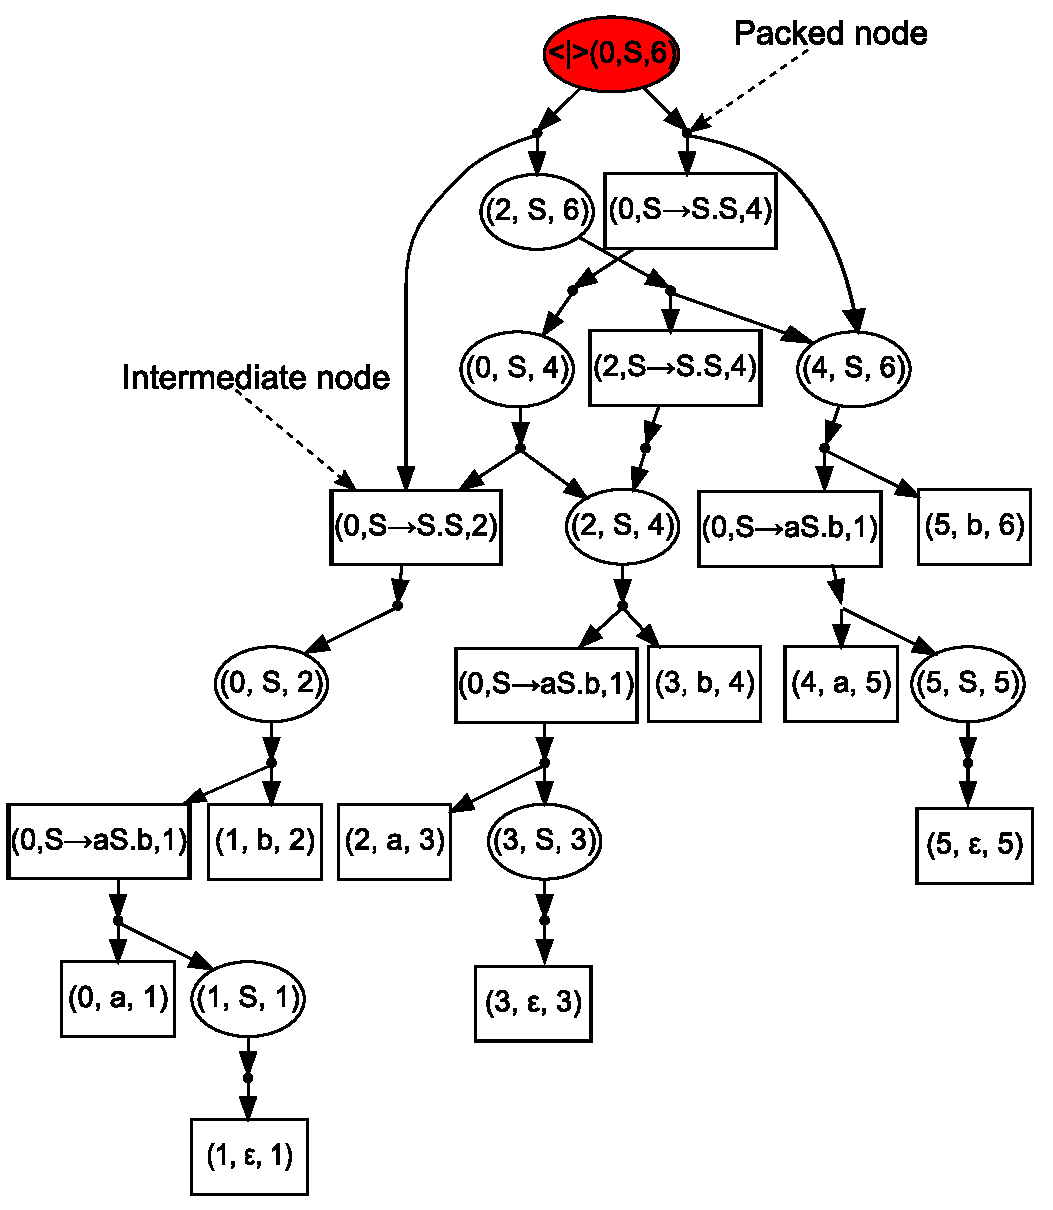
\includegraphics[width=\textwidth]{dot/Brackets.pdf}
        \caption{SPPF}
        \label{sppf}        
    \end{subfigure}
    ~
    \begin{subfigure}[b]{0.3\textwidth}
        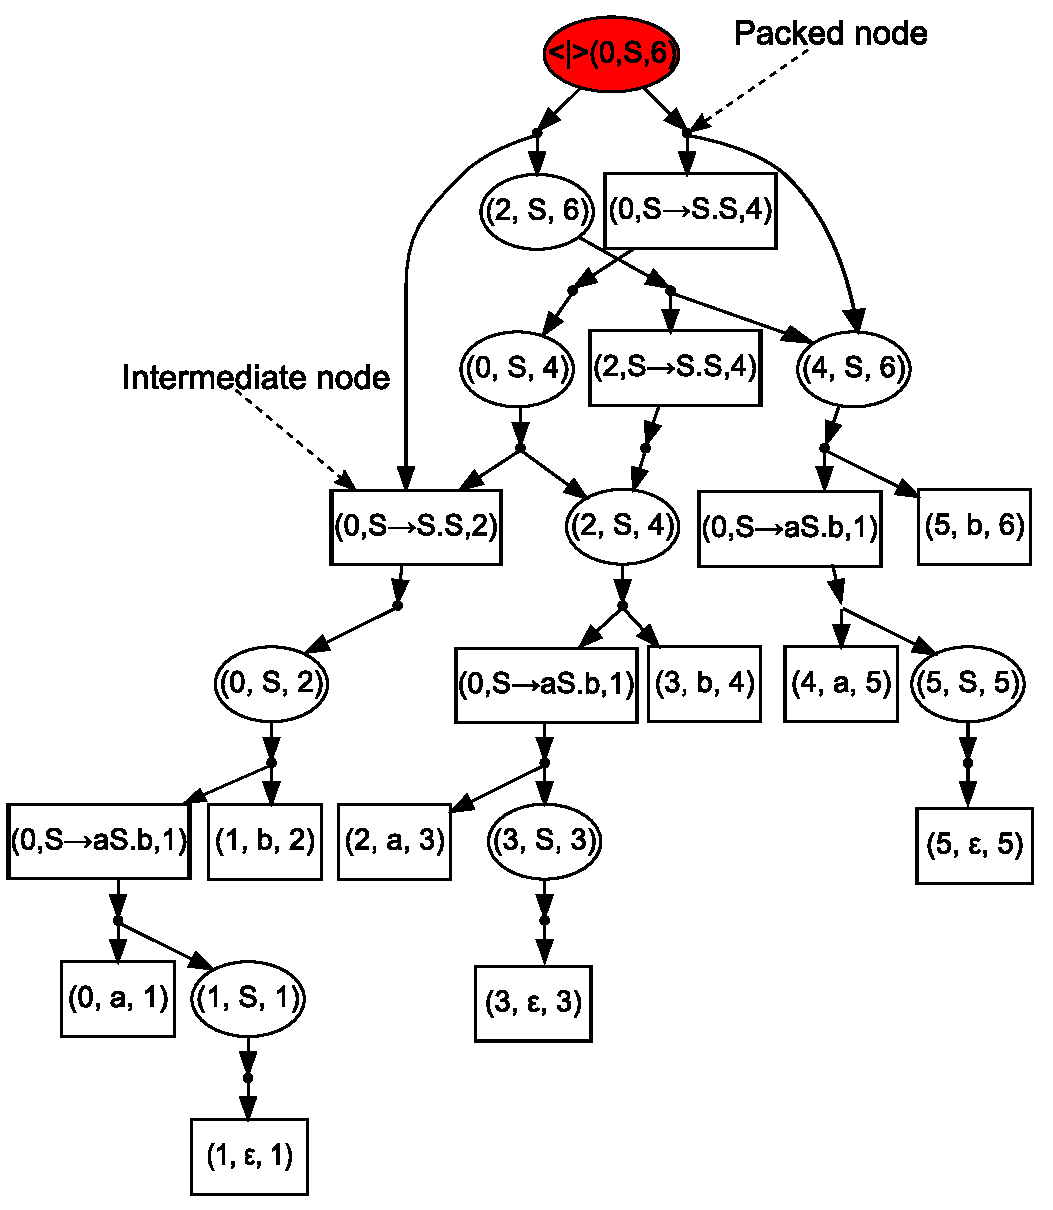
\includegraphics[width=\textwidth]{dot/Brackets.pdf}
        \caption{Tree for derivation 1}
        \label{tree1}        
    \end{subfigure}
    ~
    \begin{subfigure}[b]{0.3\textwidth}
        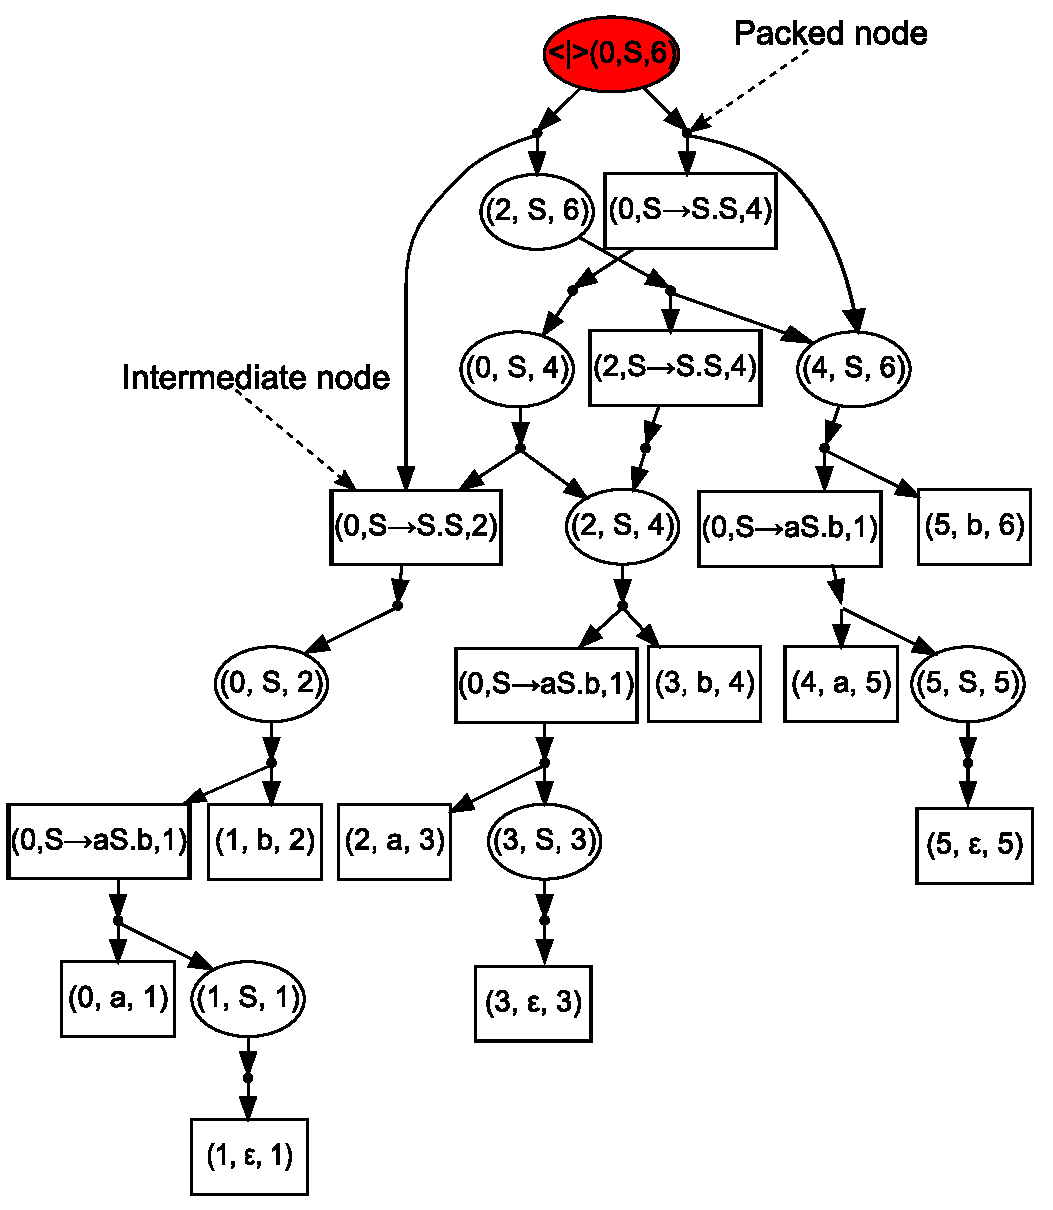
\includegraphics[width=\textwidth]{dot/Brackets.pdf}
        \caption{Tree for derivation 2}
        \label{tree2}        
    \end{subfigure}
    \caption{SPPF for sentence \textbf{\texttt{"(1)(2)(3)"}} and grammar $G_0$}
    \label{sppfSample}
    \end{center}                
\end{figure*}

Binarised SPPF can be represented as a graph where each node has one of four types: 

\begin{itemize}
    \item terminal node with label $(i,T,j)$;
    \item nonterminal node with label $(i,N,j)$;
    \item intermediate node with label $(t,i,j)$ where $t$ is a grammar slot;
    \item packed node with label $(N : \gamma \cdot, k)$;
\end{itemize}
, and one of nodes can be marked as 'root' --- node for start nonterminal.

Further in our examples we will remove redundant intermediate and packed nodes from SPPF to simplify it and decrease size of structure.

\subsection{GLL-based graph parsing}
%(!!!!!Нужен какой-то переход или рассказ про то, как мы в виде графа представляем вход!!!!!!11)
In order to use GLL for graph parsing we need only use graph vertices as position in input. After that we should modify \textbf{Processing} function such that 

\begin{algorithm}[h]
\begin{algorithmic}[1]
\caption{Control functions}
\label{mainFunctions}
\Function{processing}{}
  \State{$dispatch \gets true$}
  \Switch{$L$}
  \Case{$(X \rightarrow \alpha \cdot x \beta)$ where $x = input[i + 1])$}
       \If{$cN = dummyAST$} 
          \State{$cN \gets \Call{getNodeT}{i}$} 
       \Else 
          \State{$cR \gets \Call{getNodeT}{i}$}
       \EndIf
       \State{$i \gets i + 1$}
       \State{$L \gets (X \rightarrow \alpha x \cdot \beta)$}
       \If{$cR \neq dummy$}
          \State{$cN \gets \Call{getNodeP}{L, cN, cR}$} 
       \EndIf
  \EndCase
  \Case{$(X \rightarrow \alpha \cdot x \beta)$ where $x$ is nonterminal}
       \State{$v \gets$ \Call{create}{$(X \rightarrow \alpha x \cdot \beta), v, i, cN$}}
       \State{$slots \gets \bigcup_{e \in input.OutEdges(i)} pTable[x][e.Token]$}
       \ForAll{$L \in slots$}
          \State{\Call{add}{L,v,i,dummy}} 
       \EndFor
  \EndCase
  \Case{$(X \rightarrow \alpha \cdot )$}
       \State{\Call{pop}{v,i,cN}} 
  \EndCase
  \Case{$\_$}
       \State{final result processing and error notification} 
  \EndCase
  \EndSwitch
\EndFunction

\end{algorithmic}
\end{algorithm}



We implement some optimizations:~\cite{FastPracticalGLL}

We also use binarised SPPF for result representation which allow to simplify query debugging and result exploration. (!!!!!!А что это  зачем?!!!!!!!)
In our case more then one root may be specified. For example, look at picture!!!! 
We 

$\mathbb{P}:G, M, StartVset, FinalVSet \rightarrow SPPF$
In details, main function input is graph $M$, set of start vertices $V_s\subseteq V$, set of final vertices $V_f\subseteq V$, grammar $G_1$.
Output is Shared Packed Parse Forest (SPPF)~\cite{SPPF} --- finite data structure which contains all derivation trees for all paths in $M$, $\Omega(p) \in L(G_1)$ and allows to reconstruct any of paths implicitly.
As far as we can specify sets of start and final vertices, our solution can find all paths in graph, all paths from specified vertex, all paths between specified vertices. 
Also SPPF represents a structure of paths in terms of derivation which allow to get more useful 
information about result. 
Binarized SPPF is at most cubic in terms of result size. 
Any path can be extracted in the linear time.

A bit more on correctness.!!!!!
